\documentclass[14pt]{article}
\usepackage{url}
\usepackage{hyperref}
\usepackage{amsmath}
\usepackage{mathtools}
\usepackage{extsizes}
\usepackage{titling}
\usepackage{siunitx}
\usepackage{graphicx}
\usepackage[shortlabels]{enumitem}
\usepackage[margin=0.75in]{geometry}
\usepackage{indentfirst}
\usepackage{caption}

\newcommand{\bd}{\textbf}

\setlength{\droptitle}{-5em} 

\title{Exam 2}
\author{Mitchell Meier}
\date{\today}

\begin{document}

\maketitle

\subsection*{Problem 1}

\subsubsection*{a.}
\begin{enumerate}[(i)]

\item
The most appropriate distribution that can be used to model STAT 3113 scores from Section A is a normal distribution, according to its AIC score

\item
The mean parameter, $\mu$ is estimated to be 89.666304 \\
The standard deviation parameter, $\sigma$, is estimated to be 2.7653256 \\
The variance parameter, $\sigma^2$ is estimated to be 7.647025674 \\

\item
The most appropriate distribution that can be used to model STAT 3113 scores from Section B is a weibull distribution, according to its AIC score

\item
The mean parameter, $\mu$ is estimated to be 79.9657 \\
The standard deviation parameter, $\sigma$, is estimated to be 1.53 \\
The variance parameter, $\sigma^2$ is estimated to be 2.34129 \\
The scale parameter, $\alpha$, is estimated to be 80.650259 \\
The shape parameter, $\beta$, is estimated to be 66.269092 

\item
The probability that a randomly picked student from Section A scores more than 86 marks is $1 - 0.092451 = 0.907549$, or 90.75 percent 

\begin{figure}[h]
\centering
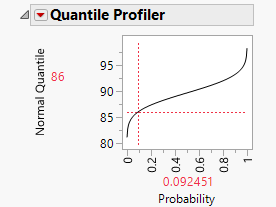
\includegraphics{exam2/1v.png}
\end{figure}

\pagebreak

\item
The probability that a randomly picked student from Section B scores less than 86 marks is $1$, or 100 percent 

\begin{figure}[h]
\centering
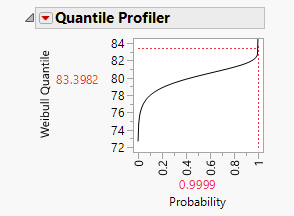
\includegraphics{exam2/1vi.png}
\end{figure}

\item
The lowest score you can achieve and still be in the top 5 percent of Section A would be a score of 94.22 percent 

\begin{figure}[h]
\centering
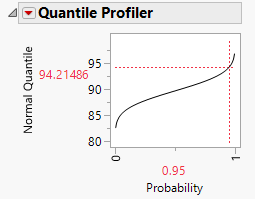
\includegraphics{exam2/1vii.png}
\end{figure}

\item
The lowest score you can achieve and still be in the top 5 percent of Section B would be a score of 82.20 percent 

\begin{figure}[h]
\centering
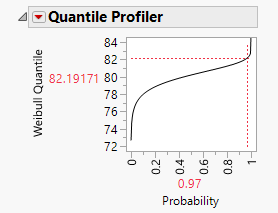
\includegraphics{exam2/1viii.png}
\end{figure}

\end{enumerate}

\subsubsection*{b.}
\begin{enumerate}[(i)]

\item
The most appropriate distribution that can be used to model failure times of the bearings is a weibull distribution, according to its AIC score

\item
The mean parameter, $\mu$ is estimated to be 4459.2 \\
The standard deviation parameter, $\sigma$, is estimated to be 2293.35 \\
The variance parameter, $\sigma^2$ is estimated to be 5259442 \\
The scale parameter, $\alpha$, is estimated to be 5033.1405 \\
The shape parameter, $\beta$, is estimated to be 2.0364645

\item
90 percent of the bearings would have failed at the time value equal to 7580.608 hours

\begin{figure}[h]
\centering
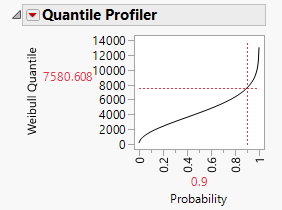
\includegraphics{exam2/1biii.png}
\end{figure}

\item
The probability that a randomly selected bearing last more than 8000 hours is is $1 - 0.923422 = 0.076578$, or 7.7 percent 

\begin{figure}[h]
\centering
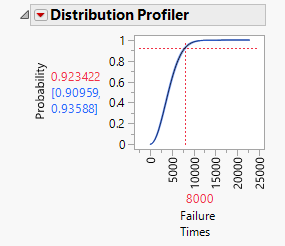
\includegraphics{exam2/1biv.png}
\end{figure}

\end{enumerate}


\subsection*{Problem 2}

\begin{enumerate}[(a)]
\item
\begin{enumerate}[1.]
\item
The population parameter given is the mean, $\mu$, of time spent watching TV each week by students at Missouri S\&T (individually), and the $\mu$ = 8 hours

\item
$H_0 : \mu = 8$ \\
$H_1 : \mu \neq 8$

\item
With a sample size of $n = 25$ \\
sample mean of $\bar{x} = 8$ \\
sample standard deviation of $s = 2.5$ \\ 
and $90$\% confidence interval, our JMP output is as follows: \\

\item
Conclusion

\end{enumerate}
\begin{enumerate}[1.]

\item
The population parameter given is the mean, $\mu$, of time an artifical heart's battery pack needs to be recharged and the $\mu$ = 4 hours \\
The population standard deviation, $\sigma$, is given as 0.2 hours

\item
$H_0 : \mu = 4$ \\
$H_1 : \mu \neq 4$

\item
With a sample size of $n = 16$ \\
sample mean of $\bar{x} = 4.1$ \\
population standard deviation of $\sigma = 0.2$ \\ 
and $90$\% confidence interval, our JMP output is as follows: \\

\item
Conclusion

\end{enumerate}

\end{enumerate}

\pagebreak

\subsection*{Problem 3}

\end{document}